\documentclass[acmtog,screen=true, pre-print]{acmart}
\usepackage{booktabs} % For formal tables


\usepackage[ruled]{algorithm2e} % For algorithms
\usepackage{float}
\usepackage{times}
\usepackage{latexsym}
\usepackage{amsmath}
\usepackage{tikz, pgfplots}
\usepackage{booktabs}
\renewcommand{\algorithmcfname}{ALGORITHM}
\SetAlFnt{\small}
\SetAlCapFnt{\small}
\SetAlCapNameFnt{\small}
\SetAlCapHSkip{0pt}
\IncMargin{-\parindent}

\newcommand\mycommfont[1]{\footnotesize\ttfamily\textcolor{blue}{#1}}
\SetCommentSty{mycommfont}
\SetKwProg{Fn}{def}{\string:}{end}
\SetKwFunction{CompGrid}{compute\_grid}
\SetKwFunction{CompTop}{compute\_topics}
\SetKwFunction{TpWG}{getAreaScore(documents)}
\SetKwFunction{McCmp}{min\_cell\_comp}
\SetKwFunction{SeqCom}{sequential\_computation}
\SetKwFunction{BslMth}{baseline\_method}
\SetKwFunction{Tta}{top\_topic\_aggregation}
\SetKwFunction{ldaup}{lda\_update(Cell A)}

\SetStartEndCondition{ }{}{}%
\SetKw{KwTo}{in}\SetKwFor{For}{for}{\string:}{end for}%
\newcommand{\forcond}{$document$ \KwTo{$documents$}}
\newcommand{\forconds}{$cell$ \KwTo{$grid$}}
\newcommand{\forPart}{$p$ \KwTo{$parts$}}
\newcommand{\forUp}{$i,\,cell$ \KwTo{$enumerate(grid)$}}
\newcommand{\forUpp}{$p$ \KwTo{$rest$}}
\newcommand{\forRecDiff}{$map$ \KwTo{$commonAreas$}}
\newcommand{\forRecCom}{$map$ \KwTo{$computedMaps$}}
\newcommand{\forNaive}{$page$ \KwTo{$pages$}}
\newcommand{\forNaiveCom}{$cell$ \KwTo{$squares$}}
\AlgoDontDisplayBlockMarkers\SetAlgoNoEnd\SetAlgoNoLine%

% Document starts
\begin{document}
% Title portion. Note the short title for running heads 
\title{Data Mining \& Big Data: A URL Categorization System}  

\author{Montagner Andrea}
\affiliation{%
  \institution{University of Trento, 189514}
  \city{Trento}
  \postcode{38122}
  \country{Trento}}
\author{Viglianisi Emanuele}
\affiliation{%
  \institution{University of Trento, 187270}
  \city{Trento}
  \postcode{38122}
  \country{Trento}}



\begin{abstract}
Nowadays, thanks to the spread of mobile devices, people can easily access to the internet. News and other information can be retrieved by just submitting a web request using a browser or smartphone application. From a web request it is possible to extract the topics discussed in the requested page that, together with the geographic origin of the requests (even more and more accurate thanks to mobile sensors), represents a meaningful set of data to analyze.\\
This paper will present a system able to analyze logs of web requests in order to extract the main topics for a specific geographic area taking care of both qualitative and performance aspect, in particular in avoiding costly re-computations.
\end{abstract}


%
% The code below should be generated by the tool at
% http://dl.acm.org/ccs.cfm
% Please copy and paste the code instead of the example below. 
%
%\begin{CCSXML}
%<ccs2012>
% <concept>
%  <concept_id>10010520.10010553.10010562</concept_id>
%  <concept_desc>Computer systems organization~Embedded systems</concept_desc>
%  <concept_significance>500</concept_significance>
% </concept>
% <concept>
%  <concept_id>10010520.10010575.10010755</concept_id>
%  <concept_desc>Computer systems organization~Redundancy</concept_desc>
%  <concept_significance>300</concept_significance>
% </concept>
% <concept>
%  <concept_id>10010520.10010553.10010554</concept_id>
%  <concept_desc>Computer systems organization~Robotics</concept_desc>
%  <concept_significance>100</concept_significance>
% </concept>
% <concept>
%  <concept_id>10003033.10003083.10003095</concept_id>
%  <concept_desc>Networks~Network reliability</concept_desc>
%  <concept_significance>100</concept_significance>
% </concept>
%</ccs2012>  
%\end{CCSXML}

%\ccsdesc[500]{Computer systems organization~Embedded systems}
%\ccsdesc[300]{Computer systems organization~Redundancy}
%\ccsdesc{Computer systems organization~Robotics}
%\ccsdesc[100]{Networks~Network reliability}

%
% End generated code
%


\keywords{Data Mining, Big Data, URL Categorization, Topic Modeling, Latent Dirichlet Allocation, TF-IDF}

\maketitle

% The default list of authors is too long for headers}
\renewcommand{\shortauthors}{A. Montagner, E. Viglianisi}

\section{Introduction}
Labor-intensive manual text mining approaches first surfaced in the mid-1980s \cite{cav}, but only a couple of decades later, due to technological advancements and the necessity of analyzing huge amount of data from internet, this field was enabled to advance. The Word Wide Web contains over 1 billion active websites \cite{ils} and, among them, social networks like Facebook and Twitter, in which over two billions users post their own contents like texts and images. These social networks have based their business on the user's data; which can be mined to extract information on the interests and needs of the users. Text mining can be seen as an interdisciplinary field that draws from machine learning, data mining, statistics, computational linguistic and information retrieval. This work studies a branch of text mining operation called topic modeling. Topic modeling is the process of identifying topics from a set of documents. A topic is usually represented by either a single word or a cluster of correlated words. For example the cluster of words [CO2, Trump, Global Warming] identifies the topic of pollution (Figure 1).\\ 
The methods described in this study can be also employed in many practical applications, like helping public institutions (schools, colleges, courthouses, libraries, hospitals) to better understand people's needs, or making trends analysis with respect to a geographical area for marketing and general statistics purposes.\\

	
	\begin{figure}[h]
	\center{\includegraphics[scale=.60]{images/topics}}
	\caption{Topics as cluster of correlated words}
	\end{figure}
	
	Furthermore, when approaching the analysis of logs, in this work logs of URLs, you have to work with huge amount of data, often a streaming of data, which require a lot of time, complex algorithms and many resources to be processed. The analysis of this kind of data is called 'Big Data analysis', and requires a parallel solution to the problem able to scale up to multiple cores and on a cluster of computers. This paper is divided in two sections; firstly a linear solution, focused on the qualitative aspect of the proposed algorithms to approach the problem, lastly a parallel solution, dealing with a performance aspect.

% Head 1
\section{Problem Definition}

The problem that has been approached and studied goes by the name of "URL Categorization". The problem and the proposed solutions are divided in two main steps:\\
	
\noindent{{\bfseries STEP 1:}} Having a dataset {\textit D} that represents logs of web requests and a geographic area {\textit M} where the requests took place, this study wants to extract, for each cell {\textit C} of a grid $S$x$S$ over the area M, the main topics for the area subscribed by the cell C based on the content of the web requests that took place in that area.

	
	\begin{description}
    	\item [INPUT] - A dataset of geotagged URL in M\\ 
					  - A grid of sizes S1xS1 over M
		
		\item [OUTPUT] - Main topics for each cell of the grid $S1$x$S1$.\\
	\end{description}
		
\noindent{\bfseries STEP 2:} Given the assumption that the grid that divides the map can be changed during the operations of zoom-in and zoom-out, re-compute from scratch the main topics for an area with a huge number of documents is an expensive operations. The second part of this study shifts the focus on the performances; indeed, the aim of this part is to find a topic modeling algorithm to avoid complete re-computation when changing the granularity of the grid from sizes $S1$x$S1$ to $S2$x$S2$.\\
	
	\begin{description}
		\item [INPUT] - A grid of sizes S1xS1 over M, each cell contains the main topics that were previously computed in the STEP1.\\
					  - A grid of sizes S2xS2 over M

					  
		\item [OUTPUT] - Main topics for each cell of the grid S2xS2.\\
	\end{description}	

\section{State of the art}

In the last few years, interest in URL categorization grew up considerably, as it is employed for different purposes. Companies like \emph{Cyren} \cite{cyren}, \emph{Brightcloud} \cite{bc}, started researching on this field to offer services of security web filtering, such as firewalls filtering requests on the basis of the content of the url as well as the destination domain. Vendors like \emph{SimilarWeb} \cite{sw}, \emph{CheckPoint} \cite{cp} or open source frameworks like \emph{DatumBox} \cite{db}, provide a well structured APIs for document analysis and classifications. For example, SimilarWeb has developed a Website Categorization API, which accurately classify an unknown website as one of 25 main categories and 219 sub-categories, with constantly improving results thanks to machine learning tools and statistical approaches.\\

As part of the URL categorization problem, topic modeling is a consolidated research field that improves, year by year, thanks to the multitude of active open source implementations of the latest researches. Among these, the most outstanding are \emph{BigARTM} \cite{ba} and \emph{Gensim} \cite{gensim}. 

After discovering the topic of the content pointed by the URL, our study takes into account the geographic origin of the requests to find out the main topics discussed in a specific area.
A similar analysis is performed by Social Network like Instagram, Facebook and Twitter, which uses the geolocation of users' contents in order to extract trends for specific areas. Although it is not difficult to imagine that Twitter's system for trends topics extraction is rather simple, as it is based on the number of tweets in which is present a particular keyword \emph{"\#hashtag"} in a geographic region, unfortunately, implementations of these systems are not disclosed by these companies for public use, so there is no full knowledge of how to perform a geo-localized categorization in the same way as Twitter does.

% Head 3
\section{Data Preprocessing}

This section delineates the guidelines performed in order to achieve the preprocessing of the data, from the cleaning of the dataset to the first computation of topics. The structure will be the following:\\

\begin{itemize}
	\item Dataset and URLs cleaning\\
	\item Topic modeling\\
	\item Initial grid computation\\
\end{itemize}

\subsection{Dataset and URLs cleaning}

In order to perform our topic modelling analysis, we need the contents of the documents as plain text. URL requests have to be suitable, they do not have to point to anything different from text web pages. Normally the dataset is heterogeneous, containing requests to music, images, videos other than plain html and text. The first step is thus filtering the URLs, only keeping the ones having \emph{text, html} in the \emph{'content-type'} field of the response headers. Having only the text contents of the web pages is a good start, but the problems are definitely not over. Take into consideration a web page, e.g. a news one from \emph{The Times} website: we are only interested in the main contents of the article, whereas all background fields (menus, ads) are useless for topic extraction, and have to be deleted. Due to this consideration, we decided to spend a little time and resources in cleaning the entire dataset from these useless components of pages. This task was carried out by using a tool called \emph{Boilerpipe} \cite{BP}.\\




\subsection{Topic modeling}

This study initially took into account two algorithms for topic modeling: LDA and TF-IDF. 
The first one, LDA \cite{LDA, blei}, presented in 2003 by D.Blei, A.Ng and M.Jordan is a generative statistical Bayesian model that allows to perform topic modeling and topic discovery. Its approach consists in representing every document as a mixture of topics, then extracts words with certain probabilities and to try to backtrack from the documents to find a set of topics that are likely to have generated the collection of documents  \cite{LDA, blei, echen}.

Then, there is TF-IDF (Term Frequency - Inverse Document Frequency) that is used to evaluate how relevant a term is to a document within a collection of documents. It is composed by two terms, Term Frequency (TF), that measures how frequently a term occurs in a document, and Inverse Document Frequency (IDF) which measures the portion of documents containing that term. The importance of the word increases proportionally to the number of times the word appears in the document but is offset by its frequency on the entire corpus \cite{TFIDF}.



Between these two algorithms the choice that best fits the considered problem is the LDA algorithm. The LDA algorithm, unlike the TF-IDF approach, does not require to known in advance the set of topics, which would be a big limitation, especially if the dataset is composed of a huge number of documents and potentially a huge number of different topics. The LDA approach instead, consists in extracting a fixed number of topics directly from the dataset, so that it is difficult to miss a main topic.

Moreover, to make use of the LDA approach, this paper refers to an open source implementation in Python called Gensim, designed for \emph{topic modeling}, \emph{document indexing} and \emph{similarity retrieval} with large corpora.\\

Gensim offers a set of API to perform topic modeling with the Latent Dirichlet Allocation. The module \emph{gensim.models.ldamodel} contains APIs that allows both LDA model estimation from a training corpus and inference of topic distribution on new, unseen documents \cite{gensim}. An already computed model can also be updated with new documents for online training. For topics extraction from a set \emph{D} of documents with this library, it is firstly necessary to create a suitable corpus. This is achieved through cleaning algorithms such as tokenization, stemming, and then representing the dataset using a bag-of-word model. The corpus is then used as input to create an LDA model. At this point, from the output, a set of $n$ topics, each one made of $m$ words, can be extracted. Each word is associated with a number, representing the probability of belonging to that particular topic. Topics extracted by LDA have an issue: they do not follow any particular order, so there is no way to understand how well a topic describes a set of documents. Gensim again provides methods to achieve this task: returning the {\bfseries topic distribution} for a given document from the LDA model. In this way the topics with the highest probability will be the ones that generated the most words in the document. Now that there is a measure of the relevance of a topic for a single document, it can be applied for an entire set, with the help of an algorithm (Algorithm 1) that weights the sum of the probabilities of each topic obtained over all documents.

\begin{algorithm}[h]
    \SetKwData{Left}{left}\SetKwData{This}{this}\SetKwData{Up}{up}
    \SetKwFunction{Union}{Union}\SetKwFunction{FindCompress}{FindCompress}
    \SetKwInOut{Input}{input}\SetKwInOut{Output}{output}

    \Fn{\TpWG{}}{
    \tcc{Initialize the $weight$ to 0}
    weight $\longleftarrow$ $0$\;
    \tcc{for each document retrieve the topics and weight them}
    	\For{\forcond}{
        	topic\_distr$\longleftarrow$ $getTopicDistribution$($document$)\;
        	weight = weight + $topics\_distr$\;

    	}
    \caption{Topic weighting}\label{alg1}
    }
          
\end{algorithm}




\subsection{Initial grid computation}

Thanks to the results obtained above, now it is possible to perform the last step of the pre-processing of the data: computing topics for the initial grid, which corresponds to the maximum level of granularity (or zoom) to provide.

\begin{figure}[h]
	\center{\includegraphics[scale=.30]{images/grid}}
	\center{\includegraphics[scale=.30]{images/gridBig}}
	\caption{Example of a grid division}
\end{figure}

The whole map where the URLs are located is subdivided according to the initial grid, then an LDA model is computed for each of the cells and stored. The reason for this pre-computation step is that, once the initial grid is computed, we only need to implement cell-aggregation (or zoom-out) operations. Furthermore, we assume the change of granularity can only take place according to the power of two (Figure 2).\\

This computation is carried out with the Baseline Method (Algorithm 2), which consists in computing an LDA model for each cell of the grid and obtaining the topics from it.

\begin{algorithm}
    \SetKwData{Left}{left}\SetKwData{This}{this}\SetKwData{Up}{up}
    \SetKwFunction{Union}{Union}\SetKwFunction{FindCompress}{FindCompress}
    \SetKwInOut{Input}{input}\SetKwInOut{Output}{output}
  
    \Fn{\BslMth{}}{
    	\tcc{Get the tokenized documents}
        dictionary$\leftarrow$$create\_dictionary($documents$)$\;
        corpus$\leftarrow$$create\_corpus($documents$, $dictionary$)$\;
        \tcc{Compute the LDA model}
		model$\leftarrow$$create\_lda\_model($corpus$)$\;
        topic$\leftarrow$$get\_topics($model$, $num\_topics$)$\;
		top\_topics$\leftarrow$$topics\_distr($topics$, $corpus$)$\;
    	
    \caption{Baseline Method (Data Mining)}\label{alg2}
    }
    
\end{algorithm}


\section{Data Mining Analysis}

The second part of the project deals with the changes of the granularity of the grid, with the aim of taking advantage of the previously obtained results to compute topics for the cells of the new grid. In addition, thanks to the initial assumption, which does not allow a new grid with an higher granularity, each cell of the new grid is composed by cells of the old grid. In this way, previously computed topics for each cell are used for determining new ones.\\

In order to evaluate the results of our optimized methods, we first computed the topics for each of the new cells with the Baseline Method, computing a new LDA model from scratch for each of the cells. Note that this solution does not use results of previous computations and it is computationally expensive, and therefore not practical.

\subsection{Algorithms}

Besides the \emph{Baseline Method}, two more practical ways of resolution have been developed:  

\begin{itemize}
	\item lda.update
	\item Top\_Topic Aggregation\\
\end{itemize}

\subsubsection{lda.update}
	This exploits the method \\\emph{lda\_model.update(}new\_crp\emph{)} provided by Gensim's module \\\emph{gensim.models.ldamodel} \cite{gensim}. Its behaviour consists in updating an already trained model ("base\_model") with new unseen corpus. This means that only a portion of the map will be re-computed, bringing a speed-up of performances. 


\begin{algorithm}
    \SetKwData{Left}{left}\SetKwData{This}{this}\SetKwData{Up}{up}
    \SetKwFunction{Union}{Union}\SetKwFunction{FindCompress}{FindCompress}
    \SetKwInOut{Input}{input}\SetKwInOut{Output}{output}
  
    \Fn{\ldaup{}}{
    	\For{\forUp}{
    	\tcc{select the cell with the higher number of documnts}
        base\_cell$\leftarrow$$cellMaxDoc($A.$getInnerCells())$\;
        \tcc{take the base model (already computed)}
        base\_model$\leftarrow$base\_cell$getModel()$\;
        \tcc{get the unseen corpus for the base\_model}
        unseen\_corpus$\leftarrow$A.$getCorpus()$$\,-\,$
        	base\_cell.$getCorpus()$\;
        \tcc{update the base\_model}
        model$\leftarrow$base\_model.$update($unseen\_corpus$)$\;
        \tcc{extract topics}
        topics$\leftarrow$$getTopics($model$, $ num\_topics$)$\;
        \tcc{get the main topic for the entire area}
        top\_topics$\leftarrow$$topic\_distr($topics$, $A.$getCorpus())$\;
    	}
    \caption{lda.update}\label{alg3}
    }
    
    \end{algorithm}
    
    Even though there is a saving in the re-computation due to the portion considered as "base\_cell", whose model is reused from previous computations, a partial re-computation of the model is performed as the remaining corpus of the new cell has to be added to the "base\_cell" model ("base\_model"). In order to maximize the performances of this method, the best choice is to pick as "base\_cell", among the previously computed cells composing the new one, the cell with the higher number of documents.\\

	\subsubsection{Top\_topic Aggregation}
	
	Here the idea is to pre-compute once the LDA model of the entire map (global model), asking for a large number of topics which holds for the entire area instead of for a sub-area. Then, in order to compute the topics for a cell C, the algorithm computes the \emph{top\_topic distributions} of the corpus of each subcell with respect to the topics extracted from the precomputed global model. Finally the topic distributions of the subcells are merged to obtain the topic distribution of the entire cell.\\

	\begin{algorithm}
    \SetKwData{Left}{left}\SetKwData{This}{this}\SetKwData{Up}{up}
    \SetKwFunction{Union}{Union}\SetKwFunction{FindCompress}{FindCompress}
    \SetKwInOut{Input}{input}\SetKwInOut{Output}{output}

    \Fn{\Tta{}}{
    \tcc{compute the top topics for each cell in the grid}
    	\For{\forconds}{
    		
    		top\_topics$\leftarrow$$[\,\,]$\;
        	\tcc{iterate over each subcell in cell}
        	\For{\forPart}{
        	\tcc{compute the topic distribution of the corpus inside the single 'part'}
        	part\_distributions$\leftarrow$$topic\_distr($lda\_map$, $
        			$part.getCorpus())$\;
            \tcc{sum the score of each topic into to obtain the final distribution top\_topic that holds for the entire cell}
            $top\_topic.merge(part\_distributions)$\;
            \tcc{save result}
            cell['top\_topic']$\leftarrow$$top\_topic$
            }
    	}
    \caption{Top\_Topic Aggregation}\label{alg4}
    }
    
    \end{algorithm}
    
In addition to the fact the LDA model is computed only once, this method also allows to save time during the evaluation of top topics: top topics of the new cell are computed by summing together the resulting topics' weights of the already computed sub-cells, instead of iterating again over all the document of the area. Note that this aggregation was not possible with the previous method since each of the cells had its own model, with its own set of topics (composed of different words).

Although \emph{Top\_Topics Aggregation} method is faster than \emph{lda\_update}, it can fail if the global model, from which we extract the topics, is computed over an area much bigger than the dimensions of a single cell and the number of extracted topics is not large enough. 
In fact, the global model might not contain topics that are only specific to a particular cell. For example, having an LDA model computed over the entire Italy, if only the region Trentino talks about \emph{"Apples"}, it is possible that the topic \emph{"Apples"} will be missing from the extracted set of the global model, due to the small ratio of documents with that topic in Italy. To minimize the probability that this problem will rise, the number $n$ of topics to extract from the global model should be chosen taking in account the number of documents in the smallest cell. It also makes sense to employ \emph{lda\_update} for those cells that contains a set of documents that it is too small to be significant for the global model.
.

\subsection{Experiments \& Results}

In the following tests, the region of interest for experiments is composed by the North-Eastern regions of Italy: Veneto, Friuli-Venezia Giulia and Trentino Alto Adige. The chosen initial (and finest) grid is composed of 16 cells, divided in 4 rows and 4 columns (Figure 3). 

\begin{figure}[h]
	\center{\includegraphics[scale=.60]{images/trentino}}
	\caption{A grid example in the area of Trentino, Veneto and Friuli}
\end{figure}

After the Baseline method is applied on the finest grid and its results are stored, both \emph{lda.update} and \emph{Top\_Topic Aggregation} methods are used in order to compute the main topics for each cell of a new grid of sizes 2x2 avoiding re-computation (Figure 4). To evaluate the results obtained with both methods, resulting top topics are compared with the one obtained through the Baseline Method. Given that topics have been extracted from different LDA models, it is necessary to define a similarity function. In this study topics are composed of 5 words, and two topics are considered to identify the same subject if they share at least three words; afterwards, a score is assigned to the method based on how many main topics are extracted that are also present in the baseline results.\\

\begin{figure}[h]
	\center{\includegraphics[scale=.60]{images/trentinored}}
	\caption{New grid}
\end{figure}


\begin{table}[h]
\centering
\caption{Similarity wrt the baseline method}
\label{tab1}
\begin{tabular}{@{}cccc@{}}
\toprule
\multicolumn{1}{l}{} & \multicolumn{1}{l}{\textit{\textbf{Number of documents}}} & \multicolumn{1}{l}{\textit{\textbf{Top topics}}} & \multicolumn{1}{l}{\textit{\textbf{lda.update}}} \\ \midrule
\textbf{Test1}       & 5056                                                     & 6                                                                
& 7                                                                \\
\textbf{Test2}       & 14329                                                      & 10                                                                & 10                                                                \\
\textbf{Test3}       & 430                                                    & 1                                                                     & 3                                                               \\ \bottomrule
\end{tabular}
\end{table}

From empirical tests, $15$ is chosen as the number of topics to extract from the global model, and $2500$ is the smallest number of documents for an area, below which is better to directly apply \emph{lda\_update}. As Table 1 shows, at the beginning two different cells are analyzed. The first test is performed taking in consideration a cell which contains of around $5000$ documents; both methods obtained a similarity around $7$ over $15$ topics. In the second test, performed over a cell of $14.000$ documents, both algorithms get instead exactly the same accuracy results of $10$ over $15$. This result is slightly better due to the higher number of documents evaluated. Finally, a third test is considered, which shows that both methods do not work as expected with a small set of documents. This happens due to the fact that topics extracted from the entire map are very different from topics computed by LDA in a small area, considering this case the LDA model does not have a large enough corpus to model the topics properly. 

These tests show both strong points and weaknesses of the proposed algorithms. On one hand, \emph{Top\_Topic Aggregation} is more suitable when the areas are large, and every area contains a non negligible portion of the whole dataset. On the other hand \emph{lda\_update} is the best choice when small increases of the dimensions of the cells are taken in consideration, so that the model will be updated with few documents. As just shown, there is no single best way of solving this problem, but rather a combination of the two methods, depending on the required application. 

This section showed a qualitative analysis of the results. The next section will take into consideration the same algorithms but focusing on the performances they have in terms of speed in a parallel solution with respect to the sequential one.\\\\



\section{Big Data Analysis}

\begin{figure*}[h]
	\includegraphics[width=\textwidth, height = 8cm]{images/mapreducefinfin}
%	\includegraphics[scale=0.3]{images/mapreduceFin}
%	\includegraphics[scale=0.5]{images/mapreduce_1}
% 	\includegraphics[scale=0.5]{images/mapreduce_2}
	\caption{Mapreduce}
\end{figure*}

The case of study of this paper is the analysis of logs of HTTP requests. The Data Mining section approaches the problem with algorithms focusing on avoiding an expensive re-computations. The implementation of the algorithm employed in the previous section are sequential and therefore not suitable in a real-life scenario, due to the large amount of data that needs to be analyzed in an acceptable time. Indeed, telecom companies may be interested in the analysis of a bigger log files much bigger than the one used to test our algorithms as well as in a live streaming analysis of the real-time requests flow. 

The proposed approaches to solve the case-of-study problem must be adapted in order to support big data analysis. The system has to be able to scale up to handle both small (chunk of a stream of data) and huge batch of data (log files, database of logs). There are some existing tools to achieve this goal, like Apache Spark and Hadoop File System, which will be presented later on. 

This part is divided into two sections: initially it is explained how the previously described approaches need to be adapted into an algorithm suited for parallel computations both in a single machine and on a cluster of computers. The second section, instead, briefly describes how to work with a streaming of data.


\subsection{Algorithm}

The previous chapter introduced three algorithms: \emph{Baseline Method}, \emph{Top\_Topic Aggregation} and \emph{lda\_update}. 

Although it is simple to parallelize the computations of the topics of the grid running the sequential algorithm in parallel for each cell of the grid, it is difficult instead parallelize the algorithms per se. In order to compute in parallel the topics of a single cell, indeed, both the Baseline and the \emph{lda\_update} method would require to maintain an always updated read and write LDA model object throughout the cluster.

Instead, \emph{Top\_topic Aggregation} is more suitable to this study due to the fact that it does not need to maintain an updated shared object. Rather, it can simply keep the access to a shared read-only LDA models, which can be distributed to workers beforehand, and accessed from the distributed file system. 


\subsection{Remarks}

The \emph{Top\_Topic Aggregation} algorithm takes as input the LDA model that holds for the whole grid, and the new grid (a partitioning of the documents) whose topics we wish to compute. Afterwards, since each cell of the new grid is composed of multiple cells of the old grid, it computes the topics distributions for each cell of the old grid and then merges these distributions together in order to obtain the topic distributions for the new cells. 

\subsection{Tools and Big Data adaptation}

The tool Apache PySpark \cite{pyspark} has been chosen due to the advantage of reusing the same modules of the data mining approach. Apache Spark is a framework which contains APIs to deal with big data, data streaming processing and cluster computing. Apache Spark supports in-memory computing and different distributed file systems, between which Apache Hadoop Distributed File System (HDFS\texttrademark) \cite{hadoop}.\\
The MapReduce programming model is exploited to adapt the \emph{Top\_Topic Aggregation} algorithm. To apply it, a pre-processing of the input is needed in order to represent the old grid as a list of tuples $(key; value)$, where the key is the index of the cell of the old grid, and the value is the set of contained documents. Each key, ID of the old grid cell, is then replaced with ID of the cell of the new grid containing it.\\ This list is the input of the MapReduce algorithm that first maps each tuple into a new tuple $(key, topic\_distributions(documents))$ computing the topic distributions for each subset of documents using the precomputed LDA model of whole grid. The tuples with the same key are then aggregated together with the reduce operation top\_topic\_merge, obtaining, for each cell of the new grid, a final topic distribution from which to extract the main topics for the cell.


\begin{algorithm}
    \SetKwData{Left}{left}\SetKwData{This}{this}\SetKwData{Up}{up}
    \SetKwFunction{Union}{Union}\SetKwFunction{FindCompress}{FindCompress}
    \SetKwInOut{Input}{input}\SetKwInOut{Output}{output}
  
    \tcc{Load the Grid}
    rdd\_grid$\leftarrow$sc.$parallelize($spark\_grid$)$\;
    \tcc{Map into <key, topic\_distributions>}
	topics$\leftarrow$rdd\_grid.$map(lambda cell: cell[$`key`$],calculate\_topic\_distibutions($lda\_map$, cell[$`corpus`$])$\;
    \tcc{Reduce by key}
    topics$\leftarrow$topics.$reduceByKey(lambda a,b: merge\_top\_topics($a$, $b$))$\;
    \tcc{Collect back results}
	topics$\leftarrow$topics.$sortByKey(True)$\;
    spark\_result$\leftarrow$topics.$collect()$\;
    	
    \caption{Spark version of \emph{Top\_Topic Aggregation}}\label{alg3}
    
\end{algorithm}

\subsection{Streaming of Data}

From the point of view of the internet provider, there's a continuous flow of http requests from several clients to servers, which is desirable to analyze immediately, instead of saving it up in a huge database for batch processing.

Apache Spark also provides streaming processing APIs, which allow to easily adapt the previously explained MapReduce algorithm to work with a continuous stream of data. (Figure 6)

In order to test the algorithm, a stream of Tweets in the interested area is captured and is streamed to Apache Spark via a socket (Algorithm 6). Spark maps the stream into a discretized stream (DStream) which is an high-level abstraction that hides the complexity of dealing with a continuous data stream and makes it as easy for programmers to treat it, as if they were working on a single RDD at a time.

The MapReduce algorithm is applied for each chunk of data (which spark obtains discretizing the stream) and, when the results for a chunk are ready, they are merged into to the topic distributions of the existing grid.

\begin{figure}[h]
%	\includegraphics[scale=.40]{images/streamingspark3}
	\includegraphics[scale=0.40]{images/streamingsparkfin}
	\caption{Spark Streaming}
\end{figure}

\begin{algorithm}
    \SetKwData{Left}{left}\SetKwData{This}{this}\SetKwData{Up}{up}
    \SetKwFunction{Union}{Union}\SetKwFunction{FindCompress}{FindCompress}
    \SetKwInOut{Input}{input}\SetKwInOut{Output}{output}
  
    \tcc{Spark receives the stream of data and map it to DStream}
    scc$\leftarrow$$StreamingContext($sc$, $30$)$\;
    lines$\leftarrow$ssc.$socketTextStream($"localhost"$, $5727$)$\;
    	
    \caption{Spark Streaming of data}\label{alg6}
    
\end{algorithm}


\subsection{Experiments \& Results}

In order to test the algorithm, the same MapReduce algorithm was tested on an $4$ cores machine with $2.4GHz$ processor and on a cluster of $4$ worker machines with $4$ cores, $2.4 GHz$ Intel Xeon processor rented on Microsoft Azure HDInsight.

Experiments show that the MapReduce algorithm has a linear complexity $O(n)$ and the performances differs by a factor that depends on the number of machines, processor and cores used.

The chart below compares the results obtained on the single-pc run with the ones from the above mentioned cluster configuration. Although the latency of the communication overhead is higher with respect to running the algorithm on a single machine, the best results are obtained, not surprisingly, from the cluster of computer. The cluster, indeed, outperformed by a factor of 3 the results of the single machine.

%\begin{figure}[h]
%	\includegraphics[scale=.40]{images/results}
%	\caption{Results}
%\end{figure}

\begin{table}[h]
\centering
\caption{{\bfseries Cluster Results (4 machines, 4 cores)}}
\label{my-label}
\begin{tabular}{@{}cc@{}}
\toprule
\textit{\textbf{Number of documents}} & \textit{\textbf{Computation time (seconds)}} \\ \midrule
\textit{20k}                          & \textit{20s}                                 \\
\textit{100k}                         & \textit{70s}                                 \\
\textit{200k}                         & \textit{153s}                                \\
\textit{500k}                         & \textit{372s}                                \\
\textit{1000k}                         & \textit{771s}                                \\ \bottomrule
\end{tabular}
\end{table}

\begin{table}[h]
\centering
\caption{{\bfseries Local Results, (1 machine, 4 cores)}}
\label{my-label}
\begin{tabular}{@{}cc@{}}
\toprule
\textit{\textbf{Number of documents}} & \textit{\textbf{Computation time (seconds)}} \\ \midrule
\textit{20k}                          & \textit{50s}                                 \\
\textit{100k}                          & \textit{272s}                                \\
\textit{200k}                          & \textit{555s}                                \\
\textit{500k}                          & \textit{1410s}                                \\
\textit{1000k}                          & \textit{2913s}                                \\ \bottomrule
\end{tabular}
\end{table}

\section{Conclusion}

In this work, it has been shown a scalable parallelized algorithm to analyze huge logs of geo-localized web requests. Thanks to this algorithm it is possible to extract main topics discussed in the geographic area described by each cell of a grid. Moreover, the described algorithms also avoid the complete re-computation of the model in cases of changes of the grid granularity due to the operations of zoom-in/zoom-out. In addition the algorithm is also applied on a streaming of tweets, which is used to simulate the scenario of dealing with a continuous stream of requests. Although in the use of the described algorithm there is a loss of accuracy whose causes are described in the previous sections, this loss is not significant, especially in large areas, considering that recomputing from scratch would be a very expensive operation.

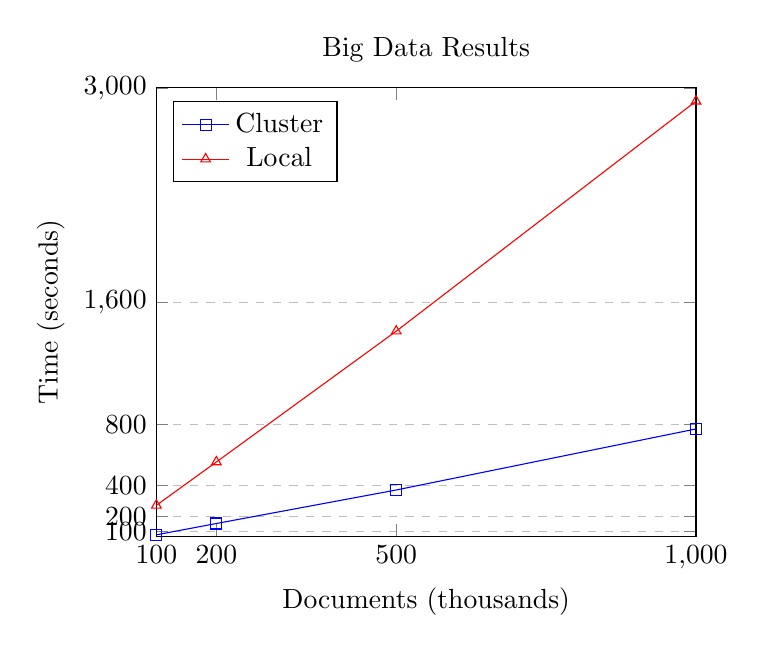
\begin{tikzpicture}
\begin{axis}[
    title={Big Data Results},
    xlabel={Documents (thousands)},
    ylabel={Time (seconds)},
    xmin=100, xmax=1000,
    ymin=70, ymax=3000,
    xtick={100,200,500,1000},
    ytick={100,200,400,800,1600,3000},
    legend pos=north west,
    ymajorgrids=true,
    grid style=dashed,
]
 
\addplot[
    color=blue,
    mark=square,
    ]
    coordinates {
    (100, 79)(200, 153)(500,372)(1000,771)};
    \addlegendentry{Cluster}

\addplot[
    color=red,
    mark=triangle,
    ]
    coordinates {
    (100, 272)(200, 555)(500,1410)(1000,2913)};
    \addlegendentry{Local}

\end{axis}
\end{tikzpicture}


% Bibliography
\bibliographystyle{ACM-Reference-Format}
\bibliography{sample-bibliography}



\end{document}
